% $Id: ExecComponents.tex,v 1.1 2008/01/31 18:04:16 dconway Exp $
%\chapter{\label{chapter:Engine}Components of the GMAT Engine}
%\chapauthor{Darrel J. Conway}{Thinking Systems, Inc.}

\setcounter{footnote}{0}

\section*{Overview of Chapters~\ref{chapter:Moderator} through \ref{chapter:Publisher}}

Mission modeling is performed in GMAT through the core numerical engine designed for the system.
This part of the architectural specification describes the classes that make up the core engine
components: the Moderator, the Factory Manager, the Configuration Manager, the Publisher, and
Sandboxes.  The purpose of each of these components is summarized in
Table~\ref{table:EngineComponents}.

\begin{table}[H]
\begin{center}
\caption{\label{table:EngineComponents}Key Elements of the GMAT Engine}
\setlength\extrarowheight{2pt}
\begin{tabular}{|p{1.4in}|p{1in}|p{3.4in}|}
\hline
Component & Notes & Description \\
\hline
\hline
Moderator & Singleton & Controls the program flow in the Engine.\\
Factory Manager & Singleton & Responsible for the creation of objects and Mission Control
Sequence commands used in the flight dynamics model.\\
Configuration Manager & Singleton & Stores and retrieves user objects created by the
Factory Manager.\\
Publisher & Singleton & Passes data generated during a run to the Subscribers that present these
data to users.\\
Sandbox & Multiple copies allowed\footnotemark & The component that manages initialization and
execution of the Mission Control Sequence when a mission is run.\\
\hline
\end{tabular}
\end{center}
\end{table}
\footnotetext{While GMAT is designed to allow more than one Sandbox, the current implementation only
uses a single Sandbox.}

\section*{Contents of the Chapters}

Each component of the engine is described in a separate chapter, structured on the following
outline:

\begin{description}
\item[Overview]

The introductory text for each chapter contains an overview of the component and its role in the
GMAT engine.

\item[Design Principles]

This section describes the motivation behind the component, along with the principles followed while
designing it.  It includes a description of patterns or other criteria used in the component design,
the roles and responsibilities handled by the component, and other design features that will help
you understand how the component fits into the GMAT engine.

\item[Design]

The design section presents the design for the component.  It starts with the class diagram
for the component, followed by descriptions of representative methods and attributes of the class
selected to help you understand its implementation.  It also provides an explanation of how the
class satisfies the roles and responsibilities identified in the preceding section, through the use
of activity and sequence diagrams.  Sometimes the details of these descriptions are better placed in
other portions of the design specification; when that happens, a summary is provided in the chapter
along with a reference to the detailed description.

\item[Usage and Modification]

This section of the chapter provides additional tips about how to use or change the component, and
includes text describing best practices for working with it.
\end{description}

% \section{\label{ModeratorOverview}The Moderator}
% 
% The core executive for GMAT is the Moderator.  The Moderator controls program flow, creating
% components through the factory manager that are then managed in the configuration manager and
%using
% these components to model missions in a sandbox.
% 
% \begin{figure}[htb]
% \begin{center}
% 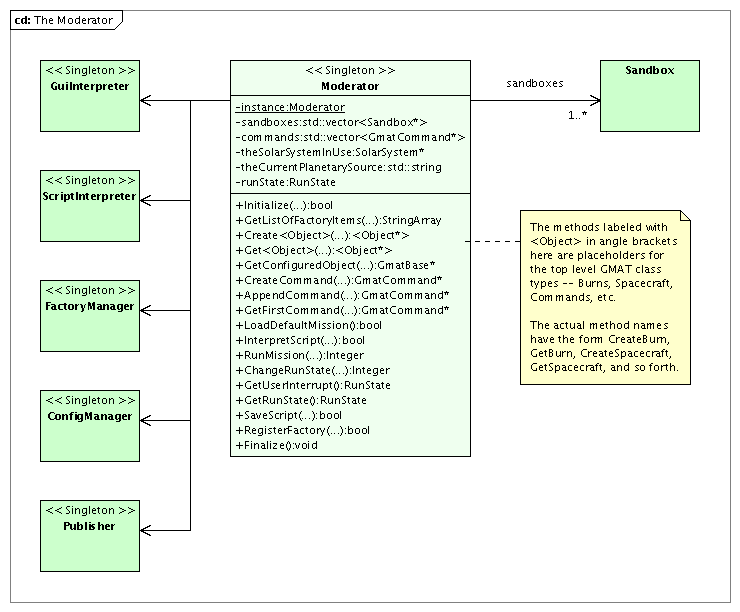
\includegraphics[370,346]{Images/TheModerator.png}
% \caption{The Moderator in its Environment}
% \label{figure:ModeratorClassDiagram}
% \end{center}
% \end{figure}
% 
% Figure ~\ref{figure:ModeratorClassDiagram} shows the Moderator, the classes it interacts with, and
% many of its key internal structures.  The interactions between the Moderator and other elements of
% GMAT's engine were presented in Chapter~\ref{chapter:TopLevel}.  The sequence diagrams presented
% there describe at a high level the interfaces to the Moderator and their usage when constructing a
% model.  The methods shown in Figure~\ref{figure:ModeratorClassDiagram} present these interfaces in
% more detail.  The following paragraphs describe these interfaces and the internal data members
%used
% by the Moderator.
% 
% \subsection{\label{section:ModeratorAttributes}Attributes and Methods of the Moderator Class}
% 
% The Moderator is a large class.  The following lists of attributes and methods provide an overview
% of the features of the class.  Interested readers should browse the code in the
% base/executive/Moderator.cpp and base/executive/Moderator.hpp, or generate the full API using
% Doxygen\cite{doxygen}, to see the full implementation details of the Moderator.
% 
% \subparagraph{\textit{Class Attributes}}
% 
% The key data members of the Moderator are the pointers to other engine elements and some core
%model
% components, as are listed here:
% 
% \begin{itemize}
% \item \textbf{static Moderator *instance}: The singleton instance of the Moderator.
% \item \textbf{std::vector<Sandbox*> sandboxes}: The sandboxes managed by the moderator.
% \item \textbf{std::vector<GmatCommand*> commands}: The Mission Control Sequences managed by this
% Moderator.  The current implementation manages one Mission Control Sequence per Sandbox.
% \item \textbf{static GuiInterpreter* theGuiInterpreter}: A pointer to the GuiInterpreter
%singleton.
% \item \textbf{static ScriptInterpreter* theScriptInterpreter}: A pointer to the ScriptInterpreter
% singleton.
% \item \textbf{ConfigManager* theConfigManager}: A pointer to the configuration manager singleton.
% \item \textbf{FactoryManager* theFactoryManager}: A pointer to the factory manager singleton.
% \item \textbf{FileManager* theFileManager}: A pointer to the file manager, a helper class used to
% manage file processing.
% \item \textbf{Publisher* thePublisher}: A pointer to the Publisher singleton.
% \item \textbf{SolarSystem* theSolarSystemInUse}: A pointer to the SolarSystem instance used when
% running a mission.
% \item \textbf{std::string theCurrentPlanetarySource}: An identifier for the current default
% planetary ephemerides source.
% \item \textbf{RunState runState}: The current state of the engine.
% \end{itemize}
% 
% \subparagraph{\textit{Engine Execution Methods}}
% 
% The methods implemented in the Moderator are broken into two categories: those used to run the
% engine, and those used to manipulate the configured objects and commands.  The following list
% describes the methods that fall into the first group.
% 
% \begin{itemize}
% \item \textbf{bool Initialize(bool isFromGui = false)}: Initializes the Moderator at the start of
% the program.  The argument to this method, isFromGui, is set to true if the Moderator was created
%in
% GMAT's GUI; otherwise, it should be set to false.  Moderator initialization is used to create the
% other singleton classes used in GMAT, some default model elements, and, when launched from the
%GUI,
% a default Mission Control Sequence.
% \item \textbf{void Finalize()}: Cleans up memory when the GMAT engine is closed down.
% \item \textbf{StringArray GetListOfFactoryItems(Gmat::ObjectType type)}: Returns a list of item
% object types, identified by generic type, that can be created in the Factory subsystem.  This
%method
% is used to determine the types of concrete objects that can be created of a given abstract type --
% for example, the list of available GmatCommands can be generated by calling this method and
% requesting the list of Gmat::COMMAND items.
% \item \textbf{bool LoadDefaultMission()}: Sets up the default mission that appears when GMAT is
% started.
% \item \textbf{void ClearAllSandboxes()}: Instructs each sandbox to clear its data and local object
% maps.
% \item \textbf{Integer RunMission(Integer sandboxNum = 1)}: This is the entry point for running a
% mission in GMAT.  The method loads the configured objects into the Sandbox, sets the Mission
%Control
% Sequence, instructs the Sandbox to initialize itself, and then to execute the control sequence.
% \item \textbf{Integer ChangeRunState(const std::string \&state, Integer sandboxNum = 1)}: Sets
% GMAT's RunState to IDLE, PAUSED, or RUNNING, based on the state description contained in the state
% string.  The sandboxNum parameter is not yet used; when multiple Sandboxes are implemented, each
% Sandbox will have its own RunState.
% \item \textbf{RunState GetUserInterrupt()}: Retrieves the RunState from the Modeartor so that the
% Sandbox can take appropriate actions in response to state changes generated by the user.  This
% method is used when the Sandbox polls the Moderator for user messages, and provides a time slice
%for
% the GUI to process user actions like selection of the Stop or Pause buttons on the toolbar.
% \item \textbf{RunState GetRunState()}: Returns the current RunState from the Moderator.
% \item \textbf{bool InterpretScript(const std::string \&filename, bool readBack, const std::string
% \&newPath)}: This method clears the current configuration and Mission Control Sequence from
%memory,
% and then  reads in and parses a script file, building a new configuration and Mission Control
% Sequence based on the contents of the script file.
% \item \textbf{bool SaveScript(const std::string \&filename, WriteMode mode = Gmat::SCRIPTING)}:
% Writes the current configuration and Mission Control Sequence to a script file, formatted in the
% mode specified by the mode flag.
% \item \textbf{std::string GetScript(WriteMode mode = Gmat::SCRIPTING)}: Writes the current
% configuration and Mission Control Sequence to a string, formatted in the mode specified by the
%mode
% flag.
% \item \textbf{Integer RunScript(Integer sandboxNum = 1)}:  Runs the current mission in the
%specified
% Sandbox.
% \end{itemize}
% 
% \subparagraph{\textit{Configured Object and Command Methods}}
% 
% The Moderator has methods to handle object and command creation for all of the user accessible
% components of the flight dynamics model, and to access these components after they have been
% created.  These facilities are used by the Interpreters during model configuration.  Future
%releases
% may also provide access to these methods from the Sandbox during a run to support object creation
% during a mission.
% 
% The configured objects are handled by type in the current implementation.  That means that there
%are
% methods with the names CreateSpacecraft and GetSpacecraft for Spacecraft objects, CreateBurn and
% GetBurn for Burn objects, and so forth for all of the configured objects created or accessed
%through
% the Moderator.  The methods used for these functions are all similar in form, so for the purposes
%of
% this chapter, they are referenced using the markers <Object> and <Object*> in the following list.
% 
% The methods used by the Moderator to create and access objects and commands are listed here:
% 
% \begin{itemize}
% \item \textbf{<Object*> Create<Object>(const std::string \&type, const std::string \&name)}:
%Creates
% an object of a given type, and assigns the specified name to that object.
% \item \textbf{<Object*> Get<Object>(const std::string \&name)}: Retrieves a named object from the
% configuration.
% \item \textbf{GmatCommand* InterpretGmatFunction(const std::string \&functionFilename)}: Builds a
% command list for a GmatFunction\footnote{GmatFunctions are not yet fully implemented.}.
% \item \textbf{GmatCommand* CreateCommand(const std::string \&type, const std::string \&name, bool
% \&retFlag)}: Creates a GmatCommand and returns it.  This method does not add commands created with
% it to the Mission Control Sequence.
% \item \textbf{GmatCommand* AppendCommand(const std::string \&type, const std::string \&name, bool
% \&retFlag, Integer sandboxNum = 1)}: Creates a GmatCommand, appends it to the Mission Control
% Sequence, and returns it.
% \item \textbf{GmatCommand* AppendCommand(GmatCommand *cmd, Integer sandboxNum = 1)}: Appends an
% existing GmatCommand to the Mission Control Sequence.
% \item \textbf{GmatCommand* GetFirstCommand(Integer sandboxNum = 1)}: Returns the head of the
%Mission
% Control Sequence for the specified Sandbox.
% \item \textbf{GmatCommand* DeleteCommand(GmatCommand *cmd, Integer sandboxNum = 1)}: Removes a
% command from the Mission Control Sequence linked list.  The removed command is returned to the
% caller for processing or deletion; the method does not call the destructor on the command.
% \item \textbf{bool InsertCommand(GmatCommand *cmd, GmatCommand *prevCmd, Integer sandboxNum~=~1)}:
% Inserts a command into the Mission Control Sequence.
% \item \textbf{GmatBase* GetConfiguredObject(const std::string \&name)}: Retrieves a configured
% object from the configuration.
% \item \textbf{bool ClearResource()}: Deletes all objects from the configuration and clears all of
% the Sandboxes.
% \item \textbf{bool ClearCommandSequence(Integer sandboxNum = 1)}: Deletes all commands from the
% Mission Control Sequence for the specified Sandbox.
% \end{itemize}
% 
% \subsection{\label{section:ModeratorStates}States of the Moderator}
% 
% The Moderator tracks the current state of the system using a parameter named runState, which is
%set
% to a value in the RunState enumeration (see Table~\ref{table:RunStateEnum}) defined in the Gmat
% namespace.  The engine states tracked in the Moderator are the IDLE, RUNNING, and PAUSED states.
% The transitions
% 
% \begin{figure}[htb]
% \begin{center}
% 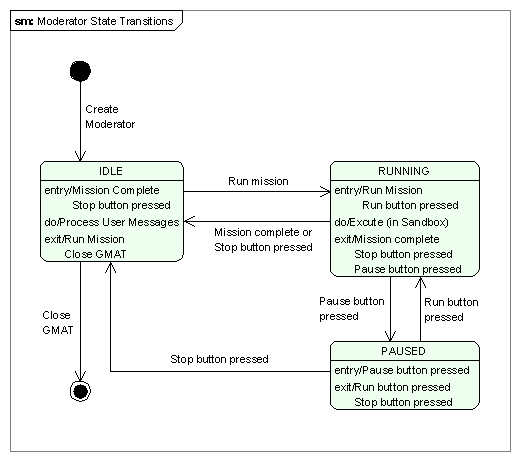
\includegraphics[260,231]{Images/ModeratorStateTransitions.png}
% \caption{State Transitions in the Moderator}
% \label{figure:ModeratorStateTransitions}
% \end{center}
% \end{figure}
% 
% Figure ~\ref{figure:ModeratorStateTransitions} shows the run state transitions tracked by the
% Moderator.  The Moderator is created with the run state set to the IDLE state.  Most of the time,
% the Moderator remains in the IDLE state, processing messages from users and managing the internal
% components of the GMAT engine\footnote{Many of the activities performed by the Moderator in the
%IDLE
% state are described in Chapter~\ref{chapter:TopLevel}.  Additional Moderator interactions with the
% other engine components are described in the appropriate sections of this document.}.
% 
% When a user executes a Mission Control Sequence, the Moderator transitions to the RUNNING state. 
%In
% this state, the Moderator performs very limited processing while the control of the system is
% managed by the sandbox that is running the mission.  The sandbox polls the Moderator for user
% activity at convenient points during the mission run.  This polling allows the Moderator to
%respond
% to user actions that either terminate the mission early or pause the mission.
% 
% If the user presses the pause button on the GUI, the Moderator transitions into the PAUSED state
% when the sandbox polls for state status.  This activity stops the mission run, but maintains data
%so
% that the run can be resumed from the point of the stop.  The user tells the Moderator to resume
%the
% run by pressing the run button on the GUI.  When the Moderator receives the run message, it
% transitions back into the RUNNING state and tells the sandbox to resume the run.
% 
% The user can terminate a run early by pressing the stop button on the GUI during a run.  This
%action
% always causes the Moderator to transition from its current state - either RUNNING or PAUSED --
%into
% the IDLE state.
% 
% \section{\label{section:FactManOverview}The Factory Manager}
% 
% Users configure GMAT by creating and using components designed to model elements or features of a
% satellite system in space.  All of these user elements are created in GMAT's factory subsystem. 
%The
% interface into this system is the FactoryManager, a singleton class that routes requests for
% specific objects into the Factory that is responsible for creating that type of object.  The
%Factory
% classes are described in Chapter~\ref{chapter:Factories}; this section describes how the
% FactoryManager interacts with the Factories and the rest of the GMAT engine to produce requested
% objects.
% 
% \subsection{\label{section:FactManAttributes}Attributes and Methods of the Factory Manager}
% 
% The Factory Manager is a singleton object, and has a fairly simple internal structure, as can be
% seen in the class diagram shown in Figure~\ref{figure:FactManClassDiagram}.  The following lists
% describe the class members shown in the figure.
% 
% \begin{figure}[htb]
% \begin{center}
% 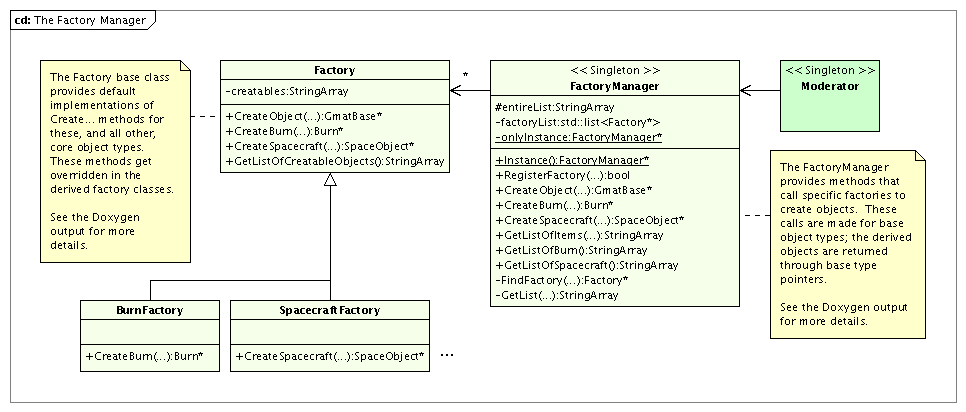
\includegraphics[455,257]{Images/TheFactoryManager.png}
% \caption{The Factory Manager in its Environment}
% \label{figure:FactManClassDiagram}
% \end{center}
% \end{figure}
% 
% \subparagraph{\textit{Class Attributes}}
% 
% The Factory Manager maintains a list of factories, and uses those factories to generate the data
% needed to respond to requests from the rest of GMAT.  There are three data members in the
% FactoryManager:
% 
% \begin{itemize}
% \item \textbf{StringArray entireList}: Array used to store the list of items requested.
% \item \textbf{std::list<Factory*> factoryList}: The array of registered factories managed by the
% Factory Manager.
% \item \textbf{static FactoryManager* onlyInstance}: The singleton pointer for the manager.
% \end{itemize}
% 
% \subparagraph{\textit{Methods}}
% 
% The Factory Manager implements methods that are used to register factories that are managed,
%access
% the lists of objects those factories can create, and access the creation methods in the factories.
% Like the Moderator, the Factory Manager provides methods that access objects by specific type.
% Those methods are described here generically, using the notation <Object> rather than explicitly
% calling out each type of object, as was done for the Moderator methods.  The Factory Manager also
% contains methods to access the class lists and object creation methods through generic calls.
% 
% The methods supported by the Factory Manager are:
% 
% \begin{itemize}
% \item \textbf{static FactoryManager* Instance()}: Access method used to get the singleton pointer.
% \item \textbf{bool RegisterFactory(Factory* fact)}: Method used to register a factory with the
% Factory Manager
% \item \textbf{GmatBase* CreateObject(const Gmat::ObjectType generalType, const std::string \\
% \&ofType, const std::string \&withName = "")}: Generic method used to create an object.
% \item \textbf{<Object*> Create<Object>(const std::string \&ofType, const std::string \&withName =
% "")}: Method used to create an object of a specific ObjectType.  Calls made through the <Object>
% methods do not need to type cast the returned objects to the appropriate object types.
% \item \textbf{StringArray GetListOfItems(Gmat::ObjectType byType)}: Method used to find the list
%of
% classes that can be created for a specific ObjectType.  This public method calls into the private
% GetList() method to find the requested data.
% \item \textbf{StringArray GetListOf<Object>()}: Method used to find the list of classes that can
%be
% created for an ObjectType.  These methods do not need the object type specifier.
% \item \textbf{Factory* FindFactory(Gmat::ObjectType ofType, const std::string \&forType)}: Method
% used to find the factory that creates instances of a specific class -- the ``forType'' class, with
%a
% specific object type.
% \item \textbf{StringArray GetList(Gmat::ObjectType ofType)}: Method used to find the list of
%classes
% that can be created for a specific ObjectType.
% \end{itemize}
% 
% \subsection{\label{section:FactoryRegistration}Registering Factories with the Factory Manager}
% 
% The Factory Manager registers factories at run time, rather than through a static list created at
% compile time.  This feature gives GMAT the ability to register factories created by users without
% forcing a recompilation of the rest of the system.  The current implementation does not support
% registration of user created factories at run time; that is a planned extension of the system. 
%The
% Factory Manager interfaces for this extension do exist in the current implementation.
% 
% \begin{figure}[htb]
% \begin{center}
% 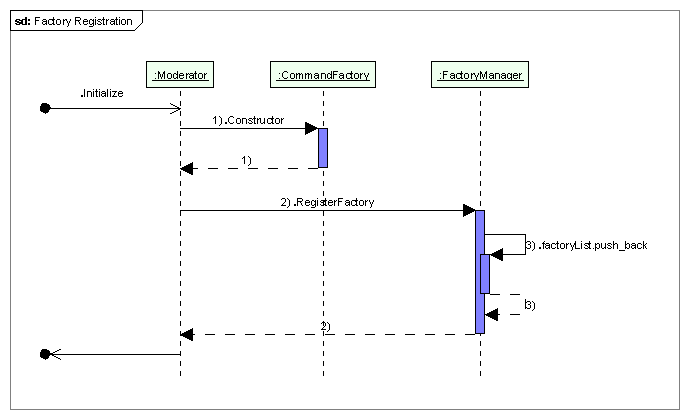
\includegraphics[345,210]{Images/FactoryRegistration.png}
% \caption{Registering a Factory}
% \label{figure:FactoryRegistration}
% \end{center}
% \end{figure}
% 
% The factory registration process, shown in Figure~\ref{figure:FactoryRegistration}, is
% straightforward.  The process starts with the Moderator.  The Moderator retrieves a pointer to the
% Factory that needs to be registered, either through object creation during initialization, or
% through the user factory registration process\footnote{The user registration process will be
% implemented in a future build.}.  In the illustrated example, the factory created is the
% CommandFactory.  The Moderator creates the CommandFactory during initialization.  It takes the
% pointer to the created factory, and passes it to the Factory Manager using the RegisterFactory
% method.  The Factory Manager receives the pointer, and adds it to the list of managed factories by
% pushing it onto the std::vector of factories.  This completes the Factory registration process.
% 
% \subsection{\label{section:CreatingObjectsWithFactMan}Object Creation through the Factory Manager}
% 
% The Factory Manager routes requests for user objects to specific factories, and passes the created
% objects back to the calling routine.  The procedure followed for this process is shown in
% Figure~\ref{figure:FactoryCreation}.
% 
% \begin{figure}[htb]
% \begin{center}
% 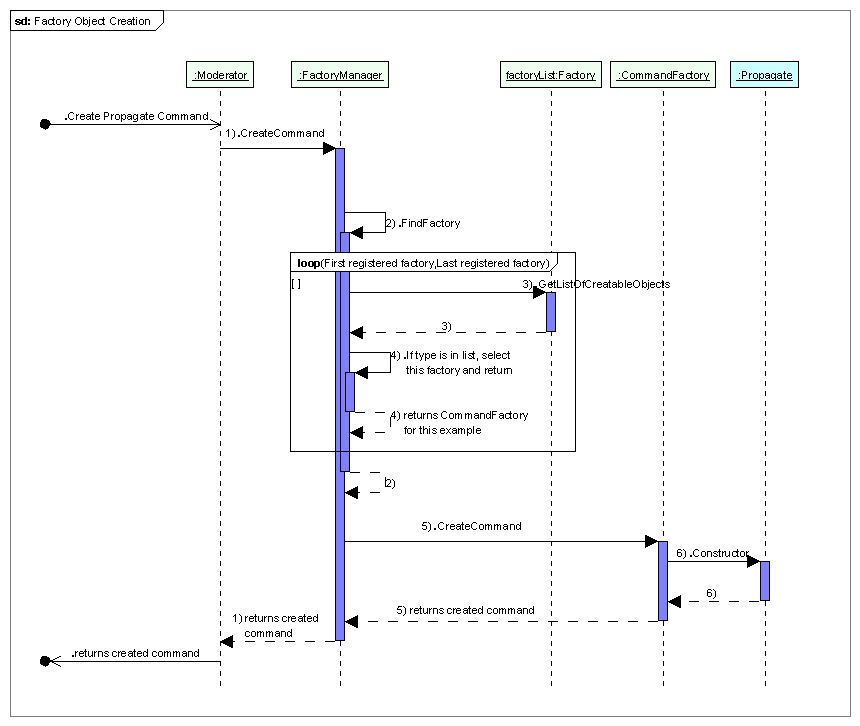
\includegraphics[430,363]{Images/FactoryObjectCreation.png}
% \caption{Creating an Object Using the Factory Subsystem}
% \label{figure:FactoryCreation}
% \end{center}
% \end{figure}
% 
% The process starts when the Moderator receives a message requesting a user object of a given type,
% optionally with a given name.  In the example shown in the figure, the request was for a Propagate
% command.  The Moderator receives the request through a call to the CreateCommand() method,
%typically
% with the syntax ``CreateCommand(``Propagate'',``'')'' for commands.  Named objects receive the
% desired name as the second parameter in this call.  The Moderator calls the Factory Manager's
% CreateCommand() method with the same parameters.
% 
% The Factory Manager calls its FindFactory() method, which locates the factory that can create
% objects of the desired type.  This method works by asking each registered factory for its list of
% creatable types.  FindFactory() checks each list returned from the registered factories until it
% finda a factory that can create the requested object type -- in this example, it searches until it
% finds a factory that can create a ``Propagate'' object.  The CommandFactory creates Propagate
% objects, so that is the factory returned from the FindFactory() method.
% 
% The factory found above is then called and asked for an object of the target type, with the name
% passed in the second parameter of the call.  The factory calls the constructor for that type of
% object -- a Propagate command object in this case -- and returns the pointer to the new object.
% This pointer is returned from the Factory Manager to the Moderator\footnote{The Moderator may
% perform other actions as well -- for instance, named objects may be passed to the Configuration
% Manager, and commands may be inserted into the Mission Control Sequence.  The Moderator actions
% taken are discussed in Chapter~\ref{chapter:TopLevel}; this discussion is only intended to provide
%a
% view into the process followed by the Factory Manager.}, and from the Moderator to the function
%that
% made the call that initiated this sequence, completing the requested task.
% 
% \section{\label{section:ConfigManOverview}The Configuration Manager}
% 
% Objects created by the Factory subsystem are stored in one of two places.  Commands are stored in
% the Mission Control Sequence.  The other objects created in the factories are stored in the
% configuration, a vector of pointers to GmatBase derivatives that is accessed by object name.  Most
% of these objects are stored directly in this vector.  Some objects are stored as objects contained
% in an object in the configuration.  An example of the latter form of object management is a
%planet,
% stored in a solar system object, which is then managed by the Configuration Manager.
% 
% \subsection{\label{section:ConfigManAttributes}Attributes and Methods of the Configuration
%Manager}
% 
% \begin{figure}[htb]
% \begin{center}
% 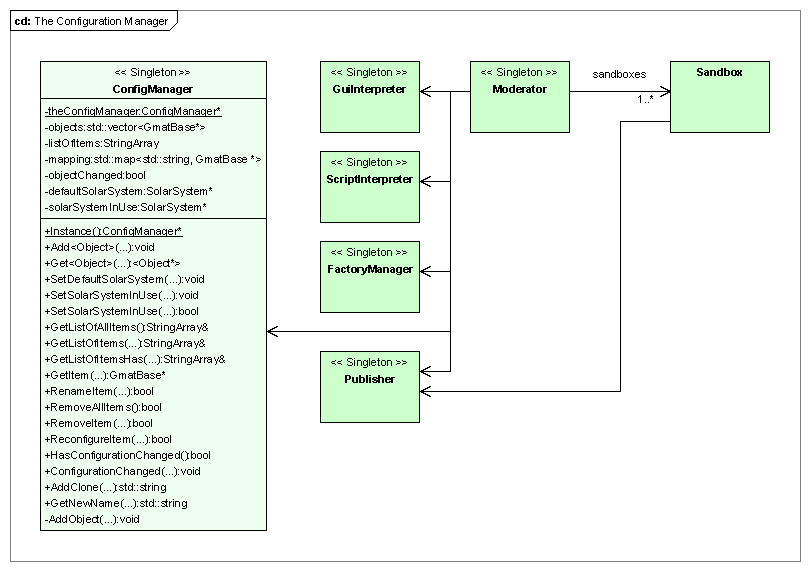
\includegraphics[405,286]{Images/TheConfigurationManager.png}
% \caption{The Configuration Manager in its Environment}
% \label{figure:ConfigManClassDiagram}
% \end{center}
% \end{figure}
% 
% The structure of the Configuration Manager is shown in Figure~\ref{figure:ConfigManClassDiagram}.
% The attributes and methods shown in this figure are described below.
% 
% \subparagraph{\textit{Class Attributes}}
% 
% The configuration is the core element managed by the Configuration Manager.  It is stored in a
% vector of GmatBase pointers named objects.  A related component, the mapping object map, keeps
%track
% of the names of the configured objects and the associated object pointers so that retrieval by
%name
% can be managed easily.  All of the Configuration Manager attributes are listed here:
% 
% \begin{itemize}
% \item \textbf{static ConfigManager* theConfigManager}: The Configuration Manager singleton.
% \item \textbf{std::vector<GmatBase*> objects}: The configuration.
% \item \textbf{StringArray listOfItems}: Array used to store lists of named items that are returned
% from some of the Configuration Manager interfaces.
% \item \textbf{std::map<std::string, GmatBase*> mapping}:  A mapping of object names to the
%pointers
% to the configured objects.  This construct simplifies retrieval of objects from the configuration.
% \item \textbf{bool objectChanged}: A flag indicating if an object in the configuration has
%changed.
% \item \textbf{SolarSystem *defaultSolarSystem}: The default solar system object.
% \item \textbf{SolarSystem *solarSystemInUse}: The current solar system selected for editing or for
%a
% run.
% \end{itemize}
% 
% \subparagraph{\textit{Methods}}
% 
% The Configuration Manager provides interfaces designed to manage insertion, access, and deletion
%of
% objects in the configuration, along with utility method that facilitate object renaming and
%queries
% into the associations between objects.
% 
% Like the Moderator and Factory Manager, the Configuration Manager has methods to add and retrieve
% objects of specific types.  These methods are listed here using the generic ``<Object>'' notation,
% rather than listing all of the specific methods.  Interested users should refer to the source code
% or Doxygen generated documentation to see the specific methods incorporated in the Configuration
% Manager.
% 
% The methods supported by the Configuration Manager are listed here:
% 
% \begin{itemize}
% \item \textbf{static ConfigManager* Instance()}:  Method used to access the Configuration Manager
% singleton.
% \item \textbf{void Add<Object>(<Object*> obj)}: Method used to add an object of a specific type to
% the configuration.
% \item \textbf{<Object*> Get<Object>(const std::string \&name)}: Used to access an object, of a
% specific type, with a specified name.
% \item \textbf{void SetDefaultSolarSystem(SolarSystem *ss)}: Sets the pointer for the default solar
% system model.
% \item \textbf{void SetSolarSystemInUse(SolarSystem *ss)}: Sets the pointer for the current solar
% system model.  In the current build of GMAT, the default and current solar system models are the
% same; this method is provided to support specification of multiple solar system models in a future
% build.
% \item \textbf{bool SetSolarSystemInUse(const std::string \&name)}: Sets the current solar system
%by
% specifying the name of a configured solar system model by name.  This method is provided to
%support
% specification of multiple solar system models in a future build.
% \item \textbf{StringArray\& GetListOfAllItems()}: Retrieves a list of the names of all of the
% objects in the configuration.
% \item \textbf{StringArray\& GetListOfItems(Gmat::ObjectType itemType)}: Retrieves a list of the
% names of all of the objects in the configuration of a specific type.
% \item \textbf{StringArray\& GetListOfItemsHas(Gmat::ObjectType type, const std::string \&name,
%bool
% includeSysParam = true)}:  Searches the configuration to determine if a specific named object is
% used by other configured objects.  For each such usage, the name of the object that uses the named
% object is added to the returned list.
% \item \textbf{GmatBase* GetItem(const std::string \&name)}:  Retrieves an object from the
% configuration and returns its pointer.
% \item \textbf{bool RenameItem(Gmat::ObjectType itemType, const std::string \&oldName, const \\
% std::string \&newName)}:  Renames an object in the configuration.
% \item \textbf{bool RemoveAllItems()}: Clears the configuration so that a new mission can be
% constructed without preserving previously created objects.
% \item \textbf{bool RemoveItem(Gmat::ObjectType type, const std::string \&name)}:  Removes a single
% object from the configuration.
% \item \textbf{bool ReconfigureItem(GmatBase *newobj, const std::string \&name)}:  Resets the
%pointer
% to a configured object with a new object pointer.
% \item \textbf{bool HasConfigurationChanged()}:  Reports the value of the objectChanged flag.
% \item \textbf{void ConfigurationChanged(bool tf)}:  Sets the value of the objectChanged flag.
% \item \textbf{std::string AddClone(const std::string \&name)}:  Clones an object and adds the
%cloned
% object to the configuration.
% \item \textbf{std::string GetNewName(const std::string \&name, Integer startCount)}:  Creates a
%new,
% unique object name based on a current name.
% \item \textbf{void AddObject(GmatBase* obj)}: Adds an object to the configuration and the object
% map.  This private method if the method that actually performs the insertion into the
%configuration
% vector.
% \end{itemize}
% 
% \section{\label{section:SandboxOverview}The Sandbox}
% 
% GMAT's model contains descriptions of the components that are used during a run and the sequence
%of
% events that needs to be executed in order to perform the run.  These pieces are assembled and
% executed in the GMAT Sandbox.  The Sandbox is created by the Moderator.  It is passed the solar
% system configuration for the run, the spacecraft and related objects used in the run, and the
% Mission Control Sequence that fires for the run.
% 
% \begin{figure}[htb]
% \begin{center}
% 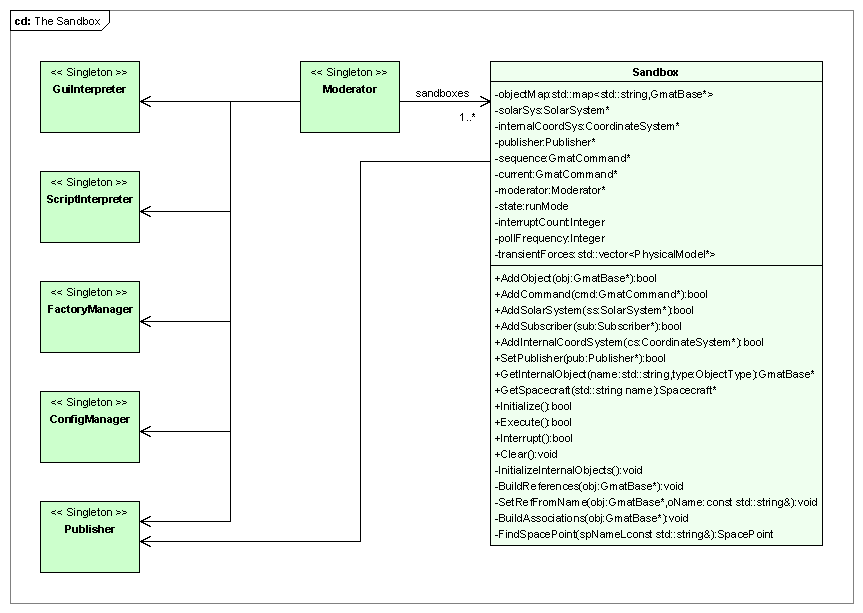
\includegraphics[432,307]{Images/TheSandbox.png}
% \caption{The Sandbox in its Environment}
% \label{figure:SandboxClassDiagram}
% \end{center}
% \end{figure}
% 
% The Sandbox manages objects internally through base class pointers, making its interfaces and
% internal data structures relatively straightforward.  The structure of the Sandbox is shown in
% Figure~\ref{figure:SandboxClassDiagram} and described in the following paragraphs.
% 
% \subsection{\label{section:SandboxAttributes}Attributes and Methods of the Sandbox Class}
% 
% The Sandbox contains the data members necessary for maintaining a local copy of the model and
% running a mission using the model.  It includes members used to communicate with the Moderator and
% Publisher, so that the processes outside of the Sandbox can control the mission run and receive
%data
% resulting from that run.  The class attributes that enable this functionality are listed here.
% 
% \subparagraph{\textit{Class Attributes}}
% 
% \begin{itemize}
% \item \textbf{std::map<std::string, GmatBase *> objectMap}: The local object map in the Sandbox,
% filled by cloning objects from the configuration.
% \item \textbf{SolarSystem *solarSys}: The solar system model used when running the Mission Control
% Sequence in the Sandbox.
% \item \textbf{CoordinateSystem *internalCoordSys}: The reference coordinate system used when
% performing conversions.
% \item \textbf{Publisher *publisher}: The GMAT publisher.
% \item \textbf{GmatCommand *sequence}: The Mission Control Sequence.
% \item \textbf{GmatCommand *current}: The current command in the Mission Control Sequence.  This
% pointer is used to traverse the linked list during a run.
% \item \textbf{Moderator *moderator}: The GMAT Moderator.
% \item \textbf{runMode state}: The current state of the Sandbox.  The Sandbox state model is
% described in Section~\ref{section:StatesintheSandbox}.
% \item \textbf{Integer interruptCount}: A counter used to track polling between the Sandbox and the
% Moderator, so that user interrupts can be processed during a run.
% \item \textbf{Integer pollFrequency}: The frequency used by the Sandbox to poll the Moderator.
% \item \textbf{std::vector<PhysicalModel *> transientForces}: A vector of forces that can be turned
% on or off in a force model during integration.
% \end{itemize}
% 
% \subparagraph{\textit{Public Methods}}
% 
% The Moderator controls model loading and the state of the Sandbox through the following public
% methods.
% 
% \begin{itemize}
% \item \textbf{bool AddObject(GmatBase *obj)}: Adds objects to the local object map.
% \item \textbf{bool AddCommand(GmatCommand *cmd)}: Sets the Mission Control Sequence.
% \item \textbf{bool AddSolarSystem(SolarSystem *ss)}: Sets the solar system model used in a run.
% \item \textbf{bool AddSubscriber(Subscriber *sub)}: Sets subscribers for the run.  This method
% registers the subscriber with the Publisher, and places the Subscriber in the local object map.
% \item \textbf{bool SetInternalCoordSystem(CoordinateSystem *ss)}: Sets the internal coordinate
% system used by the Sandbox.
% \item \textbf{bool SetPublisher(Publisher *pub = NULL)}: Sets the Publisher pointer for the
%Sandbox.
% \item \textbf{GmatBase* GetInternalObject(std::string name, Gmat::ObjectType type = \\
% Gmat::UNKNOWN\_OBJECT)}: Retrieves an object from the local object map by name.
% \item \textbf{bool Initialize()}: Initializes the Sandbox.
% \item \textbf{bool Execute()}: Runs the Mission Control Sequence.
% \item \textbf{bool Interrupt()}: Polls the Moderator to determine is a user action requires a
%state
% change in the Sandbox.
% \item \textbf{void Clear()}: Deletes clones from the local object map, clears the Sandbox's
%Mission
% Control Sequence and transient force vectors, and sets the Sandbox state to IDLE.
% \end{itemize}
% 
% \subparagraph{\textit{Private Methods}}
% 
% The Sandbox uses the following methods internally to initialize and run a mission.
% 
% \begin{itemize}
% \item \textbf{void InitializeInternalObjects()}: Sets up object references in the Sandbox's
%internal
% coordinate system and solar system.
% \item \textbf{void BuildReferences(GmatBase *obj)}: Helper method that sets all internal
%references
% for the input object.
% \item \textbf{void SetRefFromName(GmatBase *obj, const std::string \&oName)}: Finds a named object
% and sets its reference on the input object.
% \item \textbf{void BuildAssociations(GmatBase *obj)}: Finds referenced objects that need to be
% associated with the input object through cloning, creates the clones, and hands the cloned object
%to
% the owner.
% \item \textbf{SpacePoint* FindSpacePoint(const std::string \&spName)}: Finds a SpacePoint by name
% and returns it.
% \end{itemize}
% 
% \subsection{\label{section:StatesintheSandbox}State in the Sandbox}
% 
% The Sandbox maintains state information in the ``state'' member variable.  The state member is set
% to an internal enumerated value, set to one of the values of the runState enumeration designed to
% track the status of the model in the Sandbox.  This enumeration is listed in
% Table~\ref{table:SandboxRunMode}.
% 
% \begin{table}[H]
% \begin{center}
% \caption{\label{table:SandboxRunMode}Values for the Sandbox runState Enumeration}
% \setlength\extrarowheight{2pt}
% \begin{tabular}{|p{1.7in}|p{4in}|}
% \hline
% Identifier & Description \\
% \hline
% \hline
% IDLE & The Sandbox is waiting for the Moderator to prompt for a new run.  Initialized to 7001. \\
% INITIALIZED & The Sandbox has successfully initialized the local object map and the Mission
%Control
% Sequence.\\
% RUNNING & A Mission Control Sequence is executing.\\
% PAUSED & The Moderator has paused a Mission Control Sequence run.  The Sandbox is ready to resume
% the run when the Moderator triggers the run. \\
% STOPPED & The Mission Control Sequence was interrupted by the Moderator, and will not be
%resumed.\\
% RESET & The Sandbox is being reset for a new run.  This state is not used in the current
% implementation.\\
% \hline
% \end{tabular}
% \end{center}
% \end{table}
% 
% Figure~\ref{figure:SandboxStateDiagram} shows the state transitions that the Sandbox uses over the
% course of a typical session with GMAT.  The Sandbox state is initialized to the IDLE state when
%the
% Sandbox is created by the Moderator.  It remains in this state until the sandbox is needed for a
% mission run.  The sequence of events resulting in a mission run were shown in
% Figure~\ref{figure:RunningBasicScript} of Chapter~\ref{chapter:TopLevel}.  These events cause the
% sandbox transitions shown in the figure presented here.
% 
% \begin{figure}[htb]
% \begin{center}
% 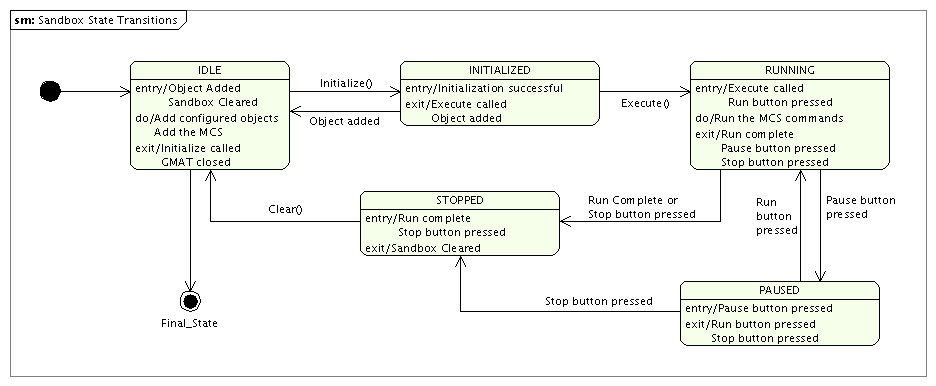
\includegraphics[455,188]{Images/SandboxStateTransitions.png}
% \caption{State Transitions in the Sandbox}
% \label{figure:SandboxStateDiagram}
% \end{center}
% \end{figure}
% 
% When the Moderator recieves a message to run a mission, it passes the configured objects and the
% Mission Control Sequence into the sandbox.  The sandbox adds the objects to the local object map
%and
% sets the sequence pointer in response to these actions, remaining in the IDLE state.  The
%Moderator
% triggers the transition from the IDLE state to the INITIALIZED state by calling the Initialize()
% method.  This method queries each object in the sandbox for referenced objects, and sets the local
% pointers to those references on each object.  If all of the local references were set
%successfully,
% the sandbox transitions to the INITIALIZED state.
% 
% \label{section:SandboxLateBinding}This binding of the reference object pointers happens inside of
% the sandbox so that the reference pointers can be set to the local clones in the sandbox.  This
%late
% binding feature is part of the GMAT design, and is incorporated in that design so that the system
% can support multiple sandboxes, and so that the system can distribute processing to multiple
% processors in future builds.
% 
% When the sandbox completes initialization, all of the components in the sandbox have their local
% references set, and the system is ready to run a Mission Control Sequence.  There are two possible
% transitions from the INITIALIZED state.  The Moderator can add additional elements to the sandbox.
% If any additional element is added, the sandbox returns to the IDLE state, indicating that object
% references have had the opportunity to be set for all of the objects in the sandbox.
% 
% The more interesting transition happens in response to a call of the Execute method from the
% Moderator.  When the Moderator calls the Execute() method, the sandbox transitions into the
%RUNNING
% state.  The sandbox starts executing the commands in the Mission Control Sequence, and runs these
% commands until either the mission runs to completion, an error occurs in the run, or the user
% interrupts processing by pressing the stop or pause button on the GUI.
% 
% If the user presses the pause button on the GUI, the sandbox transitions into the PAUSED state,
% maintaining the information required to resume the run.  From the PAUSED state, the user can
%either
% terminate the run by pressing the stop button or resume the run by pressing the run button on the
% GUI.  Pressing the stop button transitions the sandbox into the STOPPED state.  Pressing the run
% button causes a transition back into the RUNNING state, and execution of the Mission Control
% Sequence resumes from the point where the pause message was received by the sandbox.
% 
% Once the run has terminated, either by running to completion, running to an error in the sequence,
% or through a user interrupt generated by the stop button, the sandbox enters the STOPPED state. 
%In
% the STOPPED state, all of the objects in the sandbox remain in their post execution state.  This
% feature allows some limited user access to the post-run data; for example, the user can retrieve
% data at the end of execution of each command using the Command Summary panel in the GUI.  The
% sandbox's local objects remain in this post-run state until the sandbox is cleared by the
%Moderator.
% 
% The Moderator clears a sandbox by calling the Clear method.  The Clear() method destroys all of
%the
% objects in the sandbox's local object map, releases the Mission Control Sequence pointer, and
% transitions the sandbox into the IDLE state, closing the state transition loop shown
% in Figure~\ref{figure:SandboxStateDiagram}.
% 
% When GMAT closes down, the Moderator destroys the sandboxes in the system.  This last transition
% moves each sandbox from the IDLE state to the final state shown in the figure.
% 
% \subsection{\label{section:SandboxInterruptPolling}Interrupt Polling in the Sandbox}
% 
% One feature of the sandbox state transitions described above is the interaction between the
%Sandbox
% and the rest of GMAT performed to process user interrupts.  In the current implementation, the
% sandbox takes over execution when a Mission Control Sequence is running.  Each command is executed
% in order, and the sandbox moves from one command to the next in the list of commands.  Commands
%are
% executed by calling a command specific Execute() method.
% 
% Between each call to these Execute() methods, the sandbox is given the opportunity to query the
% Moderator for user interrupts.  The sandbox performs this operation periodically.  The Moderator,
% in turn, queries the GuiInterpreter for user interrupts, and the GuiInterpreter queries the GUI.
% The GUI processes any pending messages, and, if the user has presses the pause or stop button,
% sends the interrupt through the GuiInterpreter to the Moderator.  The sandbox retrieves this
% interrupt from the Moderator, and triggers the corresponding state transition, as described above.
% 
% \section{\label{section:PublisherOverview}The Publisher}
% 
% During a run users can monitor the progress through the Mission Control Sequence by watching the
% trajectory evolve in OpenGL windows, parameters change value in plot windows, and on some systems
%by
% watching data flow into output files.  GMAT uses a publish and subscribe system to drive all of
% these pipelines from the Sandbox to user viewable data sources.  The engine drives the data
%transfer
% from the Sandbox to the output objects using a singleton called the Publisher.
% 
% Data generated during a run is sent from the Sandbox containing the run to the Publisher
%singleton.
% The Publisher receives the Sandbox data, and sends the data to each Subscriber registered with the
% Publisher.  Subscribers, described in Chapter~\ref{chapter:Factories}, contain common interfaces
% that the Publisher uses to push data received from the Sandbox to the Subscribers.  Note that a
%key
% element of the publish and subscribe algorithm implemented in GMAT is that data flows in one
% direction: data is generated in the Sandbox, passed to the Publisher, and then passed from the
% Publisher to the Subscribers.
% 
% The Publisher class attributes and interfaces that enable this functionality are listed here.
% 
% \subsection{\label{section:PublisherAttributes}Attributes and Methods of the Publisher}
% 
% \begin{figure}[htb]
% \begin{center}
% 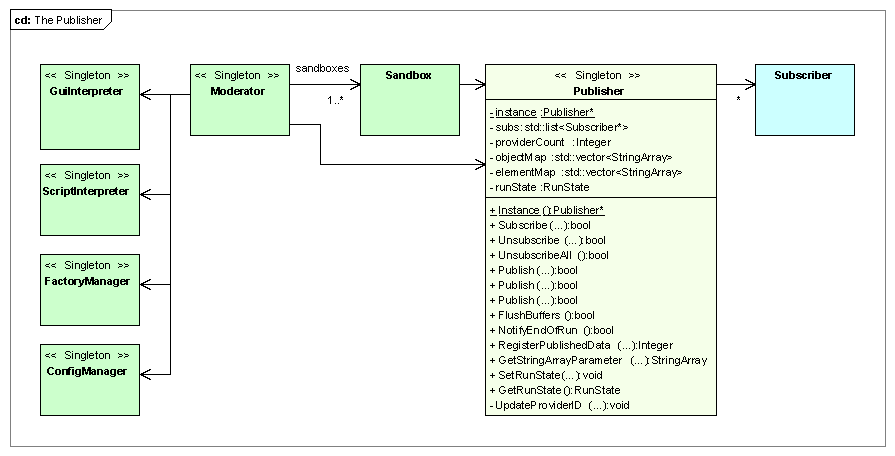
\includegraphics[445,227]{Images/ThePublisher.png}
% \caption{The Publisher in its Environment}
% \label{figure:PublisherClassDiagram}
% \end{center}
% \end{figure}
% 
% Figure~\ref{figure:PublisherClassDiagram} shows the attributes and methods incorporated in the
% Publisher.
% 
% \subparagraph{\textit{Class Attributes}}
% 
% The Publisher maintains a collection of Subscribers that are registered to receive data and
% information about the current state of GMAT in order to manage the data transfer tasks during a
%run.
%  The following attribute list is built into the Publisher to perform this maintenance:
% 
% \begin{itemize}
% \item \textbf{static Publisher *instance}:  The Publisher singleton.
% \item \textbf{std::list<Subscriber*> subs}:  The current list of Subscribers supported by the
% Publisher.
% \item \textbf{Integer providerCount}:  The number of registered data providers.
% \item \textbf{Integer currentProvider}:  The current data provider sending data to the publisher.
% \item \textbf{std::vector<StringArray> objectMap}:  List of the names of objects providing data.
% \item \textbf{std::vector<StringArray> elementMap}:  List of the names of the data elements
%provided
% to the Publisher.
% \item \textbf{Gmat::RunState runState}:  The current run state for GMAT.  The Publisher tracks the
% current run state so that Subscribers can act differently based on the current state of the
%system.
% \end{itemize}
% 
% \noindent Note that the data structures in the Publisher currently support only one set of data
% structures, mapping to a single Mission Control Sequence.  When GMAT is extended to support
%multiple
% Sandboxes, these data structures may be changed to add support for multiple Sandboxes.
% 
% \subparagraph{\textit{Methods}}
% 
% Interfaces into the Publisher are provided through the following methods:
% 
% \begin{itemize}
% \item \textbf{static Publisher* Instance()}:  Method used to access the Publisher singleton.
% \item \textbf{bool Subscribe(Subscriber *s)}:  The registration interface for the Subscribers.
% \item \textbf{bool Unsubscribe(Subscriber *s)}:  The method used to remove a Subscriber from the
% list of data receivers.
% \item \textbf{bool UnsubscribeAll()}:  Removes all Subscribers from the list of data receivers
% \item \textbf{bool Publish(Integer id, Real *data, Integer count)}:  Passes an array of Real data
% from the data source identified by id number to the Subscribers.
% \item \textbf{bool Publish(Integer id, char *data, Integer count = 0)}:  Passes an array of
% character data from the data source identified by id number to the Subscribers.
% \item \textbf{bool Publish(Integer id, Integer *data, Integer count)}:  Passes an array of Integer
% data from the data source identified by id number to the Subscribers.
% \item \textbf{bool FlushBuffers()}:  Prompts each registered Subscriber to process all received
%data
% immediately, rather than wait for an input buffer to be filled.
% \item \textbf{bool NotifyEndOfRun()}:  Tells each registered Subscriber that the Mission Control
% Sequence has finished running.
% \item \textbf{Integer RegisterPublishedData(const StringArray\& owners, const StringArray\&
% elements)}:  Registers data providers with the Publisher.  The returned value is the id for the
% registered data provider.
% \item \textbf{const StringArray\& GetStringArrayParameter(const std::string\& type)}:  Accesses
%the
% strings in the objectMap and elementMap members.
% \item \textbf{void SetRunState(const Gmat::RunState state)}:  Sets the run state for the
%Publisher.
% \item \textbf{inline Gmat::RunState GetRunState()}:  Accesses the current run state.
% \item \textbf{void UpdateProviderID(Integer newId)}:  Resets the ids for the Subscribers.
% \end{itemize}
% 
% \subsection{\label{section:PublisherStates}State Transitions in the Publisher}
% 
% \begin{figure}[htb]
% \begin{center}
% 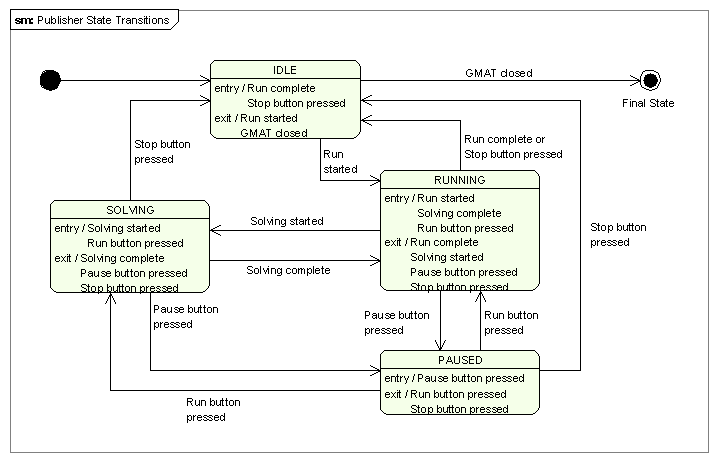
\includegraphics[359,231]{Images/PublisherStateTransitions.png}
% \caption{State Transitions in the Publisher}
% \label{figure:PublisherStateDiagram}
% \end{center}
% \end{figure}
% 
% Subscribers have the option to act differently based on the current status of the run -- for
% example, the OpenGL Subscriber can be set to show all of the published data, or only data
%published
% when the Mission Control Sequence is not running iterations through a Solver.  The Subscribers
%track
% this information through state data maintained by the Publisher.  The states tracked by the
% Publisher are shown in Figure~\ref{figure:PublisherStateDiagram}.
% 
% The Publisher starts in the IDLE state, and returns to this state when a Mission Control Sequence
% stops running.  The Publisher moves from the IDLE state to the RUNNING state when a user starts
% execution of a Mission Control Sequence.
% 
% The RUNNING state is the nominal state for the Publisher when a Mission Control Sequence is being
% executed.  The Publisher moves into the SOLVING state whenever a Solver loop is searching for a
% solution -- that is, whenever a Target command is targeting, and Optimize command is optimizing,
%or
% an Iterate command is iterating over a set of variables.  The Publisher remains in the SOLVING
%state
% until the Solver finds a solution; at that point the Publisher returns to the RUNNING state.
% 
% Users can interrupt the Mission Control Sequence by pressing either the Pause or Stop button on
%the
% GUI.  When the Pause button is pressed, the Publisher transitions into the PAUSED state.  If the
% mission resumes (i.e. if the user pressed the Run button for the paused mission), the Publisher
% returns to its previous state -- either RUNNING or SOLVING, based on the state of the Mission
% Control Sequence.  If the user presses the Stop button, the Publisher moves into the IDLE state.
